\documentclass{report}
\usepackage{fancyhdr} % Required for custom headers
\usepackage{lastpage} % Required to determine the last page for the footer
\usepackage{extramarks} % Required for headers and footers
\usepackage{graphicx} % Required to insert images
%\usepackage{lipsum} % Used for inserting dummy 'Lorem ipsum' text into the template
\usepackage{amsmath}
\usepackage{graphicx} 
%\usepackage{amsfont}
%\usepackage{amssymb}

\usepackage{multicol}
% Margins
\topmargin=-0.5in
\evensidemargin=0in
\oddsidemargin=-0.5in
\textwidth=7.5in
\textheight=9.0in
\headsep=0.25in 


\pagestyle{fancy}

%\rhead{\textbf{Marshall's Recipes}} % Top right header
%\lhead{\textbf{Curry Stir Fry}}
%\chead{ }
%\title{Curry Stir Fry}

\begin{document}
%\vspace{8mm}
%\textbf{PRELIMINARIES:}


\bigskip

\bigskip

\begin{multicols}{2}
\textbf{Ingredients}
\begin{itemize}
\item 2 yellow onion (diced)\quad (90 kCal/ 2 gP/ 0 gF/ 22 gC)
\item 2 bell pepper \quad (36 kCal/ 2 gP/ 0 gF/ 8 gC)
\item 12 eggs (scrambled)  \quad (936 kCal/ 72 gP/ 60 gF/ 12 gC)
\item 7 tbsp butter \quad (714 kCal/ 42 gP/ 35 gF/ 7 gC)
\item 12 oz package of ham steaks \quad (360 kCal/ 56 gP/ 10 gF/ 12 gC)
\item paprika 
\item garlic powder 
\item salt
\item black pepper
\item cayenne



\end{itemize}


\columnbreak
\textbf{Procedure:}
\medskip


\begin{enumerate}
\item Begin by cooking diced onion and bell pepper in 2 tbsp butter on medium heat in large pan. Cook until onions begin to turn translucent and bell peppers soften. Scamble eggs in large bowl. 


\medskip
\item Remove onion and bell pepper from skillet to plate. Scramble eggs in 6 tbsp butter. Return onion and bell pepper to pan and mix well. Season to taste. If eating immediately, heat up ham steak in pan. If meal prepping, add ham steak before heating up. 

 
\end{enumerate}
\end{multicols}


\begin{table}[h!]
  \begin{center}
    \caption{Macro totals}
    \label{tab:table1}
    \begin{tabular}{c|c|c|c} % <-- Alignments: 1st column left, 2nd middle and 3rd right, with vertical lines in between
      \textbf{Calories} & \textbf{Protein} & \textbf{Fat} & \textbf{Carbs}\\
      \hline
      2,136 kCal & 172 g & 105 g & 61 g\\
    \end{tabular}
  \end{center}
\end{table}

%\begin{center}
%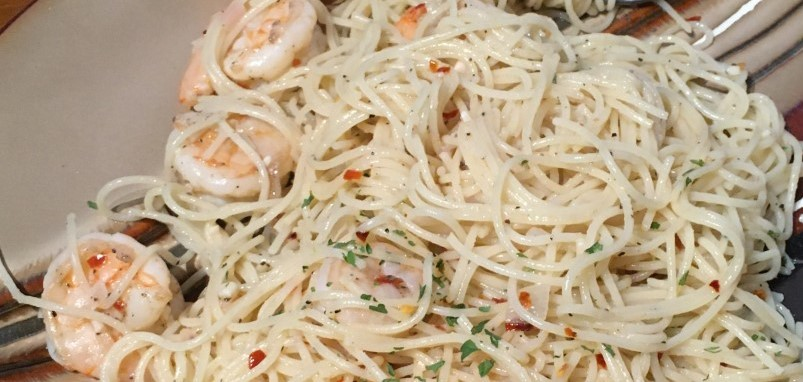
\includegraphics[scale=0.65]{Pasta/Shrimp Scampi/Shrimp Scampi.jpg}
%\end{center}


\end{document}